Nonlinear diffusion acceleration (NDA), also known as coarse-mesh finite difference, is a well-known technique applied to accelerate the scattering convergence in neutronics calculations. In multigroup neutronics problems, NDA is effective in conjunction with Gauss-Seidel (GS) iteration in energy if there is little upscattering. However, when upscattering manifests, which is common with thermal neutrons, the efficiency of GS-NDA degrades as extra iterations are required for convergence in energy \cite{park-nda}.

To remedy the issue in GS with upscattering, an energy two-grid (TG) acceleration scheme was first developed to approximate iteration error by solving a one-group diffusion-like equation with artificial material properties generated by using the scattering eigen-spectrum \cite{morel-upscat}. Later, a transport TG (TTG) method was developed that approximates the energy error using a consistent \sn\ solver in multi-D \cite{evans-upscat}. Inspired by the previous studies, we derive a TG scheme for the NDA equation with GS iteration.

\section{Background}
\subsection{Motivation}
To accelerate the convergence of transport calculations, Nonlinear Diffusion Acceleration (NDA) was developed. It pairs a lower order equation with a higher order, drift diffusion equation. As the higher order equation is not conservative, formally the method is inconsistent: The scalar flux and current may not be equal upon convergence, although they are in the limit as the spatial mesh is refined. However, second order accuracy can still be maintained with the high-order equation generally giving a more accurate shape and the conservative low-order equation giving a more accurate magnitude. The combination of the two equations has been found to be more accurate than either equation alone. \cite{morel-holo} \par
The steady-state transport equation is dependent on space, angle, and energy. It is often solved via a series of nested iterations. The various iteration methods and how they are used with each other are described in detail in \ref{sec:iterative}. The Nonlinear Diffusion Acceleration happens in the source iteration, where angle and energy are fixed. When energy is discretized into more than one energy group, an outer layer of iteration is introduced. One of the most commonly used methods for iterating over energy groups is known as Gauss-Seidel. Gauss-Siedel is guaranteed to converge eventually, however in problems with significant upscattering the time it takes to reach convergence can become arbitrarily slow. 
\par
A number of techniques to accelerate Gauss-Seidel convergence have been developed, although to our knowledge none have yet been paired with NDA.The primary techniques used in commercial transport software rely on a rebalance scheme and coarse-mesh finite-difference diffusion. Although these methods are widely used and successful for acceleration, they are very sensitive to the coarse mesh size. Rebalancing with too fine a mesh may be divergent, and an overly coarse mesh degrades performance. \cite{evans-upscat}
\par
While for standard problems, the proper mesh size is generally well understood, this is not the case for shielding problems. Adams and Morel developed an upscatter acceleration scheme known as the Two-Grid method. An estimation of the error at each Gauss-Seidel iteration is calculated using a collapsed in energy, one-group diffusion equation and energy eigenfunctions of the Gauss-Seidel iteration matrix. These make up the correction term to the scalar flux at each group which is applied at each iteration. In one dimensional calculations, Adams and Morel have demonstrated their method to be very efficient for thermal upscattering problems. \cite{morel-upscat}

\section{The Boltzmann Transport Equation}
The angular neutron flux of a reactor, $\psi$ can be described by the steady state Boltzmann Transport equation.

\begin{equation}
\begin{split}
 [\hat{\Omega} \cdot \nabla + \Sigma(\vec{r}, E)]\psi(\vec{r}, \hat{\Omega}, E) &= \chi(E) \int_0^\infty dE' \nu \Sigma_{f}(\vec{r}, E') \int_{4\pi} d\hat{\Omega}'\psi(\vec{r}, \hat{\Omega}, E') \\   &+ \int_0^\infty dE' \int_{4\pi} d\hat{\Omega}' \Sigma_s(\vec{r}, E' \rightarrow E, \hat{\Omega}' \cdot \hat{\Omega})\psi(\vec{r}, \hat{\Omega}', E')   
\end{split}
\label{eq:transport}
\end{equation}


where $\hat{\Omega}$ represents the angle; $\vec{r}$, the position vector; $E$, the energy; $\Sigma$, the total macroscopic cross-section; $\Sigma_f$, the macroscopic fission cross-section; $\Sigma_s$, the macroscopic scattering cross section; $\chi$, the energy distribution; and $\nu$, the average number of neutrons per fission. 

\subsection{Forms of the Transport Equation}
There are are several forms of the transport equaution that are of interest in the field of nuclear energy. In this work we present all methods in fixed-source form, however they can all be easily extended to $k$-eigenvalue form for criticality calculations. 

\subsubsection{Fixed Source Form}
In the fixed source form, we assume there is no fission and that there is an external neutron source, $Q$.

\begin{equation}
\begin{split}
 [\hat{\Omega} \cdot \nabla + \Sigma(\vec{r}, E)]\psi(\vec{r}, \hat{\Omega}, E) &= \\ \int_0^\infty dE' &\int_{4\pi} d\hat{\Omega}' \Sigma_s(\vec{r}, E' \rightarrow E, \hat{\Omega}' \cdot \hat{\Omega})\psi(\vec{r}, \hat{\Omega}', E')  +Q 
\end{split}
 \label{eq:transport_fixed_source}
\end{equation}

\subsubsection{$k$-Eigenvalue Form}
If the chain reaction is self-sustaining and time-independent, the reactor is known as ``critical." To maintain criticality, the asymptotic neutron distribution must not be changing over time. This behavior can be described by a parameter,  $k$, the ratio of neutrons in two successive generations. We scale $\nu$ in Eq. \ref{eq:transport} by $k$ to express the deviation from critical. This gives the following equation,

\begin{equation}
    \label{eq:transport_eigenvalue}
    \begin{split}
        [\hat{\Omega} \cdot \nabla + \Sigma(\vec{r}, E)]\psi(\vec{r}, \hat{\Omega}, E) &= \frac{\chi(E)}{k} \int_0^\infty dE' \nu \Sigma_{f}(\vec{r}, E') \int_{4\pi} d\hat{\Omega}'\psi(\vec{r}, \hat{\Omega}, E') \\ &+ \int_0^\infty dE' \int_{4\pi} d\hat{\Omega}' \Sigma_s(\vec{r}, E' \rightarrow E, \hat{\Omega}' \cdot \hat{\Omega})\psi(\vec{r}, \hat{\Omega}', E') 
    \end{split}
\end{equation}

Eq. \ref{eq:transport_eigenvalue} is simply an eigenvalue problem that with some algebraic manipulation can be thought of in the form $A\psi = \frac{1}{k} \psi$ and solved via standard eigenvalue solvers. 

\section{Useful Approximations}
In this work we are primarily concerned with the fixed source form of the transport equation, although all of our methods can be used with the eigenvalue form by replacing the fixed source $Q$ with $\frac{1}{k}\nu\Sigma_f$. For ease we assume our scattering and fixed sources are isotropic, which gives the following form

\begin{equation}
\begin{split}
 [\hat{\Omega} \cdot \nabla + \Sigma(\vec{r}, E)]\psi(\vec{r}, \hat{\Omega}, E) &= \\  \int_0^\infty \frac{1}{4\pi} &\Sigma_s(\vec{r}, E' \rightarrow E)  dE' \int_{4\pi} d\hat{\Omega}'\psi(\vec{r}, \hat{\Omega}', E')  + \frac{1}{4\pi}Q 
\end{split}
 \label{eq:transport_isotropic_scattering}
\end{equation}


This equation gives the angular flux. To find the scalar flux, $\phi$, we must integrate over all directions.
\begin{equation}
    \phi(\vec{r}, E) = \int_{4\pi} \phi(\vec{r}, \hat{\Omega}, E) d \Omega.
\end{equation}

\subsection{The Diffusion Equation}
To simplify even further, we derive another approximation. Assuming all neutrons have the same energy, consider the neutron balance within an infinitesimal volume centered at a point, $r$. Under steady state conditions, neutron conservation requires

\begin{equation}
    \textit{neutrons leaking out} + \textit{neutrons absorbed} = \textit{source neutrons emitted}.
\end{equation}
We describe the neutrons leaking out as the rate of the current, $J$, in all directions, the neutrons absorbed is the absorption cross section times the scalar flux, $\Sigma_a\phi$, and the source neutrons are represented by the source variable, $Q$. 
\begin{equation}
    \vec{\nabla}\cdot \vec{J}(\vec{r}) + \Sigma_a(\vec{r})\phi(\vec{r}) = Q(\vec{r})
\end{equation}
Using Fick's Law which relates the current to the flux, $\vec{J}(\vec{r}) = -D(\vec{r})\vec{\nabla}\phi(\vec{r})$ where $D = 1/3\Sigma_t$, we get the diffusion approximation

\begin{equation}
\begin{split}
 - \nabla \cdot D(\vec{r})\nabla\phi(\vec{r}) &+ \Sigma_a \phi(\vec{r}) = Q(\vec{r}).
\end{split}
\label{eq:diffusion_fixed_source}
\end{equation}

While the diffusion equation is much easier to solve, due to the assumptions made in the Fick's Law approximation, it is not valid near boundaries where material properties change dramatically, near localized sources, or in strongly absorbing media. 

\subsection{Nonlinear Diffusion Accelration}
This work presents an acceleration to a method known as Nonlinear Diffusion Acceleration. It reformulates the transport equation as a correction the Diffusion equation and uses a two step process to solve. For reference, we repeat the derivation of the low-order NDA equation found in \cite{morel-holo} with small modifications assuming no fission source and vacuum boundary conditions. Consider the first order, one-group, fixed-source, steady-state \sn transport equation with isotropic scattering. 

  \begin{equation}
  \vec{\Omega}\cdot \vec{\nabla} \psi \left(\vec{r}\right)+ \Sigma_{\mm{t}}\left(\vec{r}\right)\psi = \frac{1}{4 \pi} \Sigma_{\mm{s}}\left(\vec{r}\right) \phi\left(\vec{r}\right) + \frac{1}{4 \pi} Q\:.
  \end{equation}
Integrate over all angles to obtain the zeroth moment equation
\begin{equation}
  \vec{\nabla} \cdot \vec{J} + \Sigma_a\phi  =  Q
  \label{eq:zeroth_moment_1g}
  \end{equation}
where $\vec{J} = \int_{4\pi} \vec{\Omega}\psi$ and $\Sigma_a$ is the absorption cross section.   Now consider the first moment equation:
  \begin{equation}
  \vec{\nabla} \cdot P + \Sigma_t J = 0
  \end{equation}
where $\vec{\nabla} \cdot P =  \int_{4\pi} \vec{\Omega} \vec{\Omega} \cdot \vec{\nabla} \psi$. It can be rewritten as: 

  \begin{equation}
  J= -\frac{1}{\Sigma_t} \vec{\nabla} \cdot P. 
  \end{equation}
  By adding and subtracting the diffusion coefficient, $D = \frac{1}{3\Sigma_t}$, times the gradient of the flux, it takes the form of a correction to Fick's Law. 
  \begin{equation}
  J = -D \vec{\nabla} \phi + D \vec{\nabla} \phi - \frac{1}{\Sigma_t} \vec{\nabla} P \\
  = -D \vec{\nabla} \phi - \vec{\textbf{D}} \phi
  \label{eq:fick_corr_1g}
  \end{equation}
  where 
 \begin{equation}
  \vec{\textbf{D}} (\psi) = \frac{\int_{4\pi} [\frac{1}{\Sigma_t} \vec{\Omega}_\mrm \vec{\Omega}_\mrm \cdot \vec{\nabla}\psi^{ho}_\mrm] - D \vec{\nabla} \phi^{ho}}{\phi^{ho}}.
  \label{eq:drift_vector}
  \end{equation} 
Where $\psi^{ho}$ indicates the solution of the higher order equation. Plugging \eqref{eq:fick_corr_1g} into \eqref{eq:zeroth_moment_1g} we have the following NDA equation:
  \begin{equation}
  \vec{\nabla}\cdot(-D \vec{\nabla} \phi - \vec{\bf D} \phi) + \Sigma_a \phi = Q \:. \label{eq:NDA_1g}
  \end{equation}
  
 
\subsection{Self-Adjoint Angular Flux}
In calculating the drift vector in the NDA equations, we use the scalar flux calculated by a ``higher-order equation." In this case, we will be using the Self-Adjoint Angular Flux Equation (SAAF) \cite{saaf} as our higher order equation, which is a reformulation of the transport equation that is more suitable for numerical linear solvers. 

The monoenergetic version of the Self-Adjoint Angular Flux equation appropriate for $S_n$ calculations is as follows:
\begin{equation}
    - \vec{\Omega} \cdot \vec{\nabla}\frac{1}{\Sigma_t}\vec{\Omega} \cdot \vec{\nabla} \psi + \Sigma_t \psi = \Sigma_s\phi + Q - \vec{\Omega} \cdot \vec{\nabla} \frac{(\Sigma_s\phi + Q)}{\Sigma_t}
    \label{eq:SAAF}
\end{equation}
Where $\vec{\Omega}$ are the angles, $\Sigma_t$ is the total cross section, $\psi$ is the angular flux, $\Sigma_s$ is the scattering cross section, $\phi$ is the scalar flux, and $Q$ is the fixed source.

\subsection{Coupling NDA and SAAF}
In this work, we use SAAF as the higher order equation and NDA to accelerate. The implementation of the algorithm is outlined below:

\begin{enumerate}
    \item Intitialize system, by setting $\vec{\textbf{D}}$ to 0 and solving \eqref{eq:NDA_1g} to get $\phi^0$ 
    \item Loop Until Convergence:
        \begin{enumerate}
            \item Solve \eqref{eq:SAAF} for $\psi^l$ using $\phi^{l-1}$ on RHS.
            \item Calculate drift vector, \eqref{eq:drift_vector}, using $\psi^l$
            \item Solve \eqref{eq:NDA_1g} for $\phi^l$
            \item Check $\phi^{l-1}, \phi^l$ for convergence
        \end{enumerate}
    \item Return $\phi$
\end{enumerate}

% \begin{algorithm}
% \caption{Nonlinear Diffusion Acceleration}
% \begin{algorithmic}
%     \State Initialize system, setting drift vector, $\vec{\textbf{D}}$, to 0
%     \State Solve the low-order linear system to get $\phi^0$
%     \While{$res > tol$}
%         \State Use low-order solution as $\phi$ in high-order system
%         \State Solve higher order system for, $\psi^l$
%         \State Calculate drift vector and boundary coefficients using $\psi^l$
%         \State Solve low-order system for $\phi^l$
%         \State $res \gets || \phi^l - \phi^{l-1} ||$
%     \EndWhile
%     \State \textbf{return} $\phi$
% \end{algorithmic}
% \label{alg:NDA}
% \end{algorithm}



\section{Methods of Discretization}
The angular flux, $\psi$, is a function of space, angle, and energy. In the solution process, each one of those dimensions is discretized. There are several choices that have to be made when choosing discretizations. In this work, we endeavor to show equation forms that are discretization agnostic as well as showing formulations unique to the particular discretization methods we chose to implement. 

\subsection{Angular Discretization}

Angular discretization on the left hand side of \eqref{eq:transport} is handled via the discrete ordinates ($S_N$) method, a finite-element collocation method \cite{Lathrop1965}. We assume the sources are isotropic and do not perform any additional expansion, however they can be expanded via Spherical Harmonics and the methods will still hold. 

The $S_N$ method evaluates the equation at number of discrete angles or ``ordinates" and then sums over all angles with their given weights to perform a quadrature. To choose quadrature points, an octant of the unit sphere is discretized into several levels. At each level several nodes are chosen.We use a Gauss-Chebyshev angular quadrature set, which can be thought of as a product set, combining a one dimensional Gaussian Quadrature along the polar angles and an equally-weighted Chebyshev quadrature along the azimuthal angles \cite{jarrel-thesis}.

\begin{figure}
    \centering
    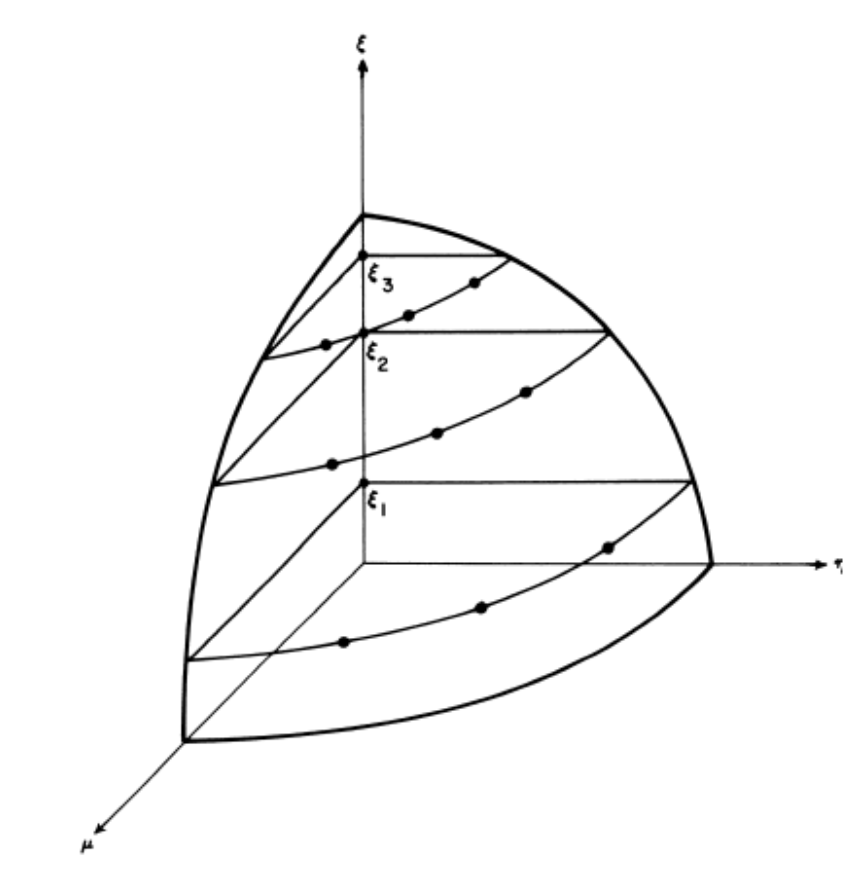
\includegraphics[width=.5\textwidth]{fig/SNPoints.png}
    \caption{Equally-Weighted Gauss-Chebyshev Quadrature Points \cite{Lathrop1965}}
    \label{fig:SN}
\end{figure}


The discretized, steady-state, $S_N$ transport equation is given as follows,

 \begin{equation}
  \vec{\Omega}_\mrm \cdot \vec{\nabla} \psi_\mrm \left(\vec{r}\right)+ \Sigma_{\mm{t}}\left(\vec{r}\right)\psi_\mrm = \frac{1}{4 \pi} \Sigma_{\mm{s}}\left(\vec{r}\right) \phi\left(\vec{r}\right) + \frac{1}{4 \pi} Q
  \label{eq:transport-angular}
 \end{equation}
where $\mrm$ is the angular index and $\phi = \sum\limits_{\mrm=1}^M \omega_\mrm \psi_m$.

\subsection{Energy Discretization}
In our treatment of energy, we divide the full energy spectrum into several energy groups. By convention, the highest energy group is given the index, 1, with the index number going up until it reaches the lowest energy group. In expanding to multiple energy groups, we must take into account scattering from one group, $\rg'$ to another, $\rg$, denoted as $\rg' \rightarrow \rg $. The cross sections we use in our experiments were generated using NJOY from ENDF data.

The energy discretized, steady-state, transport equation is

 \begin{equation}
  \vec{\Omega} \cdot \vec{\nabla} \psi_\rg \left(\vec{r}\right)+ \Sigma_{\mm{t}, \rg}\left(\vec{r}\right)\psi_\rg = \frac{1}{4 \pi} \sum\limits_{\rg'=1}^{G}\Sigma_{\mm{s}, \rg' \rightarrow \rg}\left(\vec{r}\right) \phi_\rg\left(\vec{r}\right) + \frac{1}{4 \pi} Q_\rg.
  \label{eq:transport-energy}
 \end{equation}


\subsection{Spatial Discretization}
In this work, we choose to discretize in two dimensions, assuming uniformity in the third, however all formulations could be extended to be truly 3D. Spatial discretization methods for the transport equation is usually performed using commonly known differential equation discretization techniques such as the finite difference, finite volume, or finite element methods. In this work we discretize using the finite element method (described in detail in Appendix \ref{sec:spatial}), however the form of TG-NDA given can be used with any spatial discretization. 



